% !TeX root = ../thesis.tex
\section{Background}
The background section will cover eight topics.
First insurance policies in general will be explained.
Following this, the mathematics employed in this project will be covered. 
This consists of Thiele's differential equation and the fourth-order Runge-Kutta method for solving differential equations.

After the mathematics is covered, the technologies utilized will be presented.
First general information on parallelization and the potential benefits of using the GPU compared to the CPU will be explained.
The CUDA platform and CUDA C will then be presented.
This is followed by an introduction of F\#'s meta-programming model Code Quotations which is used by Alea.cuBase to generate GPU code.
The syntax of the Actulus Calculation Specification (CalcSpec) language will then briefly be explained.
Finally, the hardware the project has been tested on will be presented.

\subsection{Life Insurance Policies and Markov-models}
A life insurance policy is a contract stating the obligations an insuring party has to an insured party in and transitioning between various finite states over many years.
Such states can include being alive and well (active), disabled, dead and more.
Transitions between states will have a certain probability, for example mortality rates for transitions between the active and dead state.
A state model such as this is also known as a continuous-time Markov-model which is used for both its expressiveness and its analyzability.

Figure \ref{fig:markovexample} shows an example of such a model with 3 states and 3 transitions between states. More or less of both are possible.
The labels between the states each have a $\mu$-function that states the probability of the transition occurring at time $t$. 
This is also known as the transition intensity.
Not all transition intensities will change over time while others such as mortality rate will.
For each change in time $t$ to $t+1$ there may be associated costs whether there is a state transition or not.

\begin{figure}[h] 
\setlength{\unitlength}{0.14in} % selecting unit length 
\centering % used for centering Figure 
\begin{picture}(20,8) % picture environment with the size (dimensions) 
 % 32 length units wide, and 15 units high. 
\put(3,6){\framebox(6,3){Active}} 
\put(13,6){\framebox(6,3){Disabled}}
\put(8,0){\framebox(6,3){Dead}} 

\put(6.2,6){\vector(1,-1){2.9}}
\put(9,7.5){\vector(1,0){3.9}} 
\put(16.2,6){\vector(-1,-1){2.9}}

\put(9.5,8.5) {$\mu_{a-di}(t)$}
\put(15,4) {$\mu_{di-d}(t)$} 
\put(4.5,4) {$\mu_{a-d}(t)$} 
\end{picture} 
\caption{Disability Term Insurance Markov-model example} % title of the Figure 
\label{fig:markovexample} % label to refer figure in text 
\end{figure} 

\subsection{Thiele's differential equation and the Runge-Kutta Method}
The goal of the computations performed in this thesis is to estimate the amount of money (reserve) required to be able to fulfil the obligations of a given life insurance plan.
Thiele's differential equation called ``the foundation of modern life insurance mathematics''\cite{bergermathematik} is a tool for determining conditional expected values in Markov models and it can be used to express a variety of life insurance policies.
The equation is expressed below in equation \ref{eq:thiele}. It assumes continuity for $V_s$, $b_s$, $\mu$ for every $t$ and consists of the following parts:

\begin{itemize}
\item $S$ is the total amount of states
\item $V_s(t)$ is the reserve at time $t$ in state $s$
\item $r_s(t($ is interest-rate at time $t$ in state $s$
\item $b_s(t)$ is the benefit paid by the insurer at time $t$ in state $s$
\item $T_s(t)$ is the possible transitions in state $s$
\item $\mu_{s,ts}(t)$ is the transition intensity from state $s$ to state $ts$
\item $b_{s,ts}(t)$ is the transition cost from state $s$ to state $ts$
\end{itemize}

\begin{equation}\label{eq:thiele}
\begin{split}
\frac{d}{dt}V_s(t) = \forall_{s\in S}r_s(t) V_s(t) - b_s(t) - \sum_{ts \in T_{s}} \mu_{s,ts}(t) (V_{ts}(t) - V_s(t) + b_{s,ts})
\end{split}
\end{equation}

To shortly summarize it, the derivative reserve for a state is for all states the current reserve times the interest-rate minus the benefit paid by the ensurer minus the transitioning costs to all possible states. 
The transitioning cost to a state is the intensity of the transition times the difference in reserves plus the cost of transitioning.

With a differential equation such as this, we need a way to approximate a result numerically. 
The Runge-Kutta method\cite{press2007numerical} is a method for integrating ordinary differential equations (ODEs) by using a trial step at the midpoint of an interval to cancel out lower-order error terms.
It works within boundaries set by a start point and end point. If the start point is greater than the end point, the algorithm works with negative step-sizes.
The common implementation uses a fixed amount of steps to reduce the inaccuracy of the method. 
Increase the amount of steps reduces the inaccuracy at the cost of increased computation.
The most common step size seen in this project is 100 by advice of Peter Sestoft.
The fourth-order version of the method can be seen below in equation \ref{eq:rk4} approximating $y$ in the step from $t$ to $t+h$. It consists of the following parts:

\begin{itemize}
\item $h$ is the size of the step. With 100 steps, the step-size would be 0.01, or -0.01 if the start point $>$ end point.
\item $f(t, e)$  is the right hand side of the given differential equation evaluated at time $t$ in an environment $e$
\item $t$ is the initial time of the step
\item $y_t$ approximated result at time t
\item $O(x)$ represents the inaccuracy of the method
\end{itemize}

\begin{equation}\begin{aligned}\label{eq:rk4}
&k_1 = h f(t, y_t)\\
&k_2 = h f(t + \frac{h}{2}, y_t + \frac{k_1}{2})\\
&k_3 = h f(t + \frac{h}{2}, y_t + \frac{k_2}{2})\\
&k_4 = h f(t + h, y_t + k_3)\\
&y_{n+1} = y_t + \frac{k_1}{6} + \frac{k_2}{3} + \frac{k_3}{3} + \frac{k_4}{6} + O(h^5)
\end{aligned}\end{equation}

%Insert graphics showing step

\subsection{Parallelization and the GPU}
Parallelization is the act of taking one large task and splitting it into smaller tasks that run concurrently (''in parallel'').
This could for example be an algorithm that initially does some computation that loops $n$ times where each iteration is independent and takes $w$ time to complete, but is altered to instead utilize $n$ tasks that each execute one iterations worth of work.
Instead of taking $w \cdot n$ time to complete, it can now be done in just $w$ time plus whatever overhead is associated with creating the tasks and dividing the work.
This is reliant on each iteration being independent, as if the iterations are dependent on each other then it can not be executed before the previous iteration completes.
Loops isn't the only way to utilize parallelization and all independent tasks can in theory be parallelized. 
Utilizing various synchronization techniques, partially dependent calculations can also harness the power of parallelization, though at the risk of increased complexity and deadlocks.
As only independent computation parallelization is utilized, other forms will not be discussed further.

Parallelization can be performed on multi-core CPUs utilizing constructs such as processes and threads, but can especially be utilized by GPUs that were designed for compute-intensive and highly parallel computations, precisely what graphics rendering is about.
This is because unlike the CPU which is specialized for data-caching and flow control, the GPU has more transistors dedicated to data processing as illustrated in green by figure \ref{cpugpu}. The figure contains Arithmetic Logic Units (ALU's, in green) responsible for logical operations and integer arithmetic, Control Units (in yellow) responsible for communication and coordination between input/output devices and various memory units (in orange) such as a memory cache and dynamic random-access memory (DRAM).

\begin{figure}[h!]
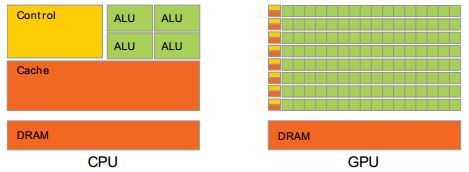
\includegraphics{cpugpu.jpg}
\caption{The GPU devotes more transistors to data processing. From the CUDA C Programming Guide \cite{nvidia2014programming}\label{cpugpu}}
\end{figure}

\subsection{The CUDA platform and CUDA C}
CUDA is NVIDIAs parallel computing platform and programming model for harnessing the power of the GPU.
The CUDA platform consists of the CUDA C and C++ language (referred to as CUDA C from this point), based on the C and C++ languages but with some alterations.
It also has parallel computing extensions for other languages such as Fortran and Python.
The CUDA Toolkit is also a part of the platform, consisting of a compiler, math libraries and tools for debugging and optimizing performance as well as guides, user manuals, API references and other documentation.

\subsubsection{CUDA Architecture}
The CUDA model is build around a hierarichal architecture of the GPU. 
At the top of the architecture is the streaming multi-processor (SM) of which a GPU can have many. 
Each SM consists of multiple CUDA cores that are used to concurrently execute a group of 32 threads known as a warp. As the SM executes the instructions in terms of warps, the total amount of threads in a block should be a multiple of the warp-size for maximum efficiency.
Each SM executes one group of threads that have access to a shared memory-space. This group of threads, which should be a multiple of warps, is called a block. 
As each SM executes a block at a time, more SMs available to the GPU will speed up the execution of the total amount of blocks. 
This also means that the amount of blocks should be a multiple of the amount of multiprocessors for maximum efficiency. %confirm

\subsubsection{Memory model}
A thread has access to memory only available to itself. This is done using registers, that are fast, as long as they're available and falling back on local memory otherwise, which is slow.
Beyond that it has access to shared memory that is available to all threads in the same block, which is fast, as well as global memory accessible to all threads in all blocks, which is slow.
There is also constant memory and texture memory both of which are fast but immutable. 
There is also a L1 and L2 cache \textbf{todo.. used for global/local memory I suppose?}.
The properties of the various memory types can be seen in table \ref{table:memorytypes}.
{\renewcommand{\arraystretch}{3}%
\begin{table}[h!]
\centering
\begin{tabular}{ | c | c | c | c | }
  \hline
           & Mutable & Speed & Cached \\ \hline
  Register & Yes     & Fast  & No     \\ \hline
  Local    & Yes     & Slow  & Yes    \\ \hline
  Shared   & Yes     & Fast  & No     \\ \hline
  Global   & Yes     & Slow  & Yes    \\ \hline
  Texture  & No      & Fast  & Yes    \\ \hline
  Constant & No      & Slow  & Yes    \\ \hline

\end{tabular}
\caption{Properties of CUDA memory types\label{table:memorytypes}}
\end{table}

%Update the above table to something more useful...
%Talk about memory throughput

\subsubsection{CUDA C}
CUDA C is mostly C with added declaration specifiers for methods and variables. The most essential declaration specifier is the \textbf{\_\_global\_\_} specifier which declares a method to be a \textbf{kernel}. Kernels are void-methods that are callable from the CPU but will be executed on the GPU. Code sample \ref{cuda_add} shows a simple kernel performing vector addition of the vectors of size $N$.

\begin{lstlisting}[language=C++, caption=CUDA C addition kernel, label=cuda_add]
__global__ void Add(float* a, float* b, float* result){
	//unique id within the kernel
	int i = threadIdx.x + blockIdx.x * blockDim.x;
	// (blockIdx always 0 in this example)
	result[i] = a[i] + b[i];
}

int main(){
	...//Initiate memory on host and device
	Add<<<1, N>>>(a, b, result); //invoke kernel on 1 block of N threads
	...//Copy back and use result, free memory as appropriate
}
\end{lstlisting}

Another thing to note is the launch-parameters of the Add-kernel which specify the amount of blocks and the amount of threads per block. A block can be organized into either one-dimensional, two-dimensional or three-dimensional grids. This can be convenient in the case of working with for example matrices, but is not utilized in this thesis and will not be covered in further detail.

CUDA C also has other declaration specifiers. \textbf{\_\_device\_\_} specifies that a method will only be compiled for the GPU (which can be referenced by kernels), \textbf{\_\_host\_\_} specifies that a method will be available for the CPU. These two specifiers can also be used together for compilation to both platforms.
Variables have the \textbf{\_\_device\_\_} qualifier, as well as \textbf{\_\_constant\_\_} to indicate it should be stored in constant memory or \textbf{\_\_shared\_\_} for shared memory.

As it is based on C, dynamic memory must be allocated using $malloc$ and subsequently de-allocated by $free$.
This operation also has to be done for the device memory using the equivalent $cudaMalloc$ and $cudaFree$.
The tediousness of this is one of the many benefits of using a modern language, but at the cost of control that could potentially decrease performance.

\subsection{F\# Code Quotations}
Code quotations is a language feature of F\# that allows one to dynamically generate abstract syntax trees from F\# expressions. It is used in particular to transform F\# to other languages, for example SQL, automatically. It can also be used to generate F\# code that can be evaluated. Code quotations support both typed and untyped expressions using $<@ ... @>$ and $<@@ ... @@>$ respectively.

For example, the expression $<@ let plusfive number = number + 5 in plusfive @>$ is automatically translated into the abstract syntax tree in figure \ref{quotationast}. As quotations only support expressions, a let declaration can not exist on its own, hence returning the function at the end (in the $in$ part of the quotation).

\begin{lstlisting}[caption=Abstract syntax tree for the example quotation expression, label=quotationast]
Let (plusfive, 
	Lambda (number, 
		Call (None, op_Addition, [number, Value (5)])
	), 
	plusfive)
\end{lstlisting}

Code quotations also allow for the mixing of quotation expressions using the splicing operators $\%$ for typed and $\%\%$ for untyped expressions as can be seen in code sample \ref{quotationsmixin}.

\begin{lstlisting}[caption=Quotation mixing, label=quotationsmixin]
let plusfive = <@ let plusfive number = number + 5 in plusfive @>
//Has type Expr<int->int>
let plus10 = <@ let plusten number = number |> %plusfive |> %plusfive in plusten @>
//Also has type Expr<int->int>
let untypedplus10 = <@@ %plus10 @@>
//Has type Expr
\end{lstlisting}


\subsection{F\# and Alea.cuBase}
F\#\cite{fsharp} is an open source, cross-platform functional programming language originating from Microsoft that runs on the .NET platform.
Alea.cuBase by QuantAlea\cite{quantalea} is a commercial language-integrated compiler for F\# that allows for CUDA development on the .NET platform.
By relying on run-time code-generation it allows for extremely extensible kernels to an extend not easily possible in CUDA C.

It utilizes F\#'s meta-programming support Code Quotations for automatic run-time generation of abstract syntax-trees that are then compiled into CUDA's Instruction Set Architecture (ISA) Parallel Thread Execution (PTX) code using Alea.cuBase's compilation API.
Code sample \ref{cubase_add} shows what a simple vector squaring-kernel could look like in F\# with Alea.cuBase.

\begin{lstlisting}[caption=Alea.cuBase square kernel, label=cubase_add]
let Square = cuda { //use the Alea.cuBase cuda workflow
  let! kernel = <@ fun (a:deviceptr<int>) (result:deviceptr<int>) ->
      let i = blockIdx.x * blockDim.x + threadIdx.x
      result.[i] <- a.[i] * a.[i] @> |> Compiler.DefineKernel
  return Entry(fun program ->
    let worker = program.Worker
    let kernel = program.Apply kernel
    //return host-execution method
    fun (a:int[]) ->
      use a = worker.Malloc(a)
      use result = worker.Malloc(Array.zeroCreate a.Length)
      kernel.Launch (LaunchParam(1, a.Length)) a.Ptr result.Ptr
      result.Gather()) //return result
}
[<EntryPoint>]
let main argv = 
  let a = [| for i in 1 .. 10 -> i |]
  use program = Square |> Compiler.load Worker.Default
  program.Run a |> Array.iter (fun e -> printfn "%d" e)
  0 //return 0 to indicate success
\end{lstlisting}

The $cuda$ workflow/computation expression (or ``monad'' for the so inclined) contains the kernel defined in a code quotations and compiled to an actual kernel, and it returns a host-side execution method that will handle allocation and de-allocation of device-side memory. 
As we are using F\#, the deallocation is handled automatically by using the $use$-keyword that automatically frees up resources once the variables referencing them are out of scope. 
The program is then loaded to a worker (a CUDA context and background-thread) in the main method compiling the PTX code to NVIDIA internal ISA code. %explain better
The program is then run using the parameters defined in the run-time method of the $cuda$ workflow (in this case, it just takes an integer array) and the result is returned to the CPU where it can be processed (in this example, the result is simply printed).

\subsection{Actulus Calculation Specification language}
The Actulus Calculation Specification language (CalcSpec) is a language for defining the differential equations that make up an insurance plan. The overall structure can be seen in code sample \ref{calcspecstructure}.


\begin{lstlisting}[caption=CalcSpec structure, label=calcspecstructure]
calculation = {
    name = <Name of calculation>,
    algorithm = { <Algorithm> },
    equations = { <Equations> },
    range = { <Range> },
    [output = "[" <Output> "]",]
    boundaryvalues = { <Boundary values> },
    expressions = { <Expressions> }
  }
\end{lstlisting}

\begin{itemize}
\item The $<Algorithm>$ will include the name of the algorithm (for example ``Runge Kutta 4'') and the parameters (for example the step-size for Runge Kutta 4) for the algorithm.
\item The $<Equations>$ describes the differential equations used by the algorithm. This is typically done by referencing functions defined in $<Expressions>$. Every component of the differential equation must describe the coefficients of the component. If coefficients are 0, they can also be described as constants (for example 0) or as an empty blocks for multi-part coefficients.
\item The $<Range>$ and $<Boundary\ values>$ are related to the differential equation described in $<Equations>$ and describes the interval in which the algorithm should solve the equation using the boundary conditions.
\item $<Output>$ is an optional declaration that specifies which parts of the calculations that should be returned. It is currently not supported in this project. %Update if added
\item $<Expressions>$ is where constants and function are defined. Functions can only take one parameter but can reference other constants and variables.
\end{itemize}

An example of the pure endowment insurance plan can be seen in code sample \ref{pe_calcspec}. 
Note that it utilizes the Dirac $delta$ function which is used to express a discontinuity point.%explain and cite

\begin{lstlisting}[caption=The pure endowment insurance plan expressed in CalcSpec, label=pe_calcspec]
calculation = 
  {
    name = 'Pure endowment',
    algorithm = { type = 'Runge Kutta 4', parameters = { stepsize = 0.01 } },
    equations = { 
        0 = { r_j = r, b_j = b0, mu_jk = { 1 = GM }, b_jk = { } },
        1 = { },
    },
    range = { from = 40, to = 0 },
    boundaryvalues = { 0 = 0 , 1 = 0 },
    expressions = {
        interestrate = 0.05,
        bpension = 1,
        pensiontime = 35,
        age = 30,
        r(t) = interestrate,
        b0(t) = bpension * delta(t - pensiontime),
        GM(t) = 0.0005 + 10 ^ (5.728 - 10 + 0.038*(age + t))
    }
  }
\end{lstlisting}

\subsection{Hardware}
%Reduce, move fluff to appendix
As the intended audience for this particular application of parallelization is fairly limited and can be expected to afford specific hardware, it has not been a concern that specific hardware may be required to run it.
The minimal requirement to run the program is a GPU of at least compute capability 2.0.
The code was only tested on the NVIDIA Tesla C2075 GPU which has the following properties:

\begin{itemize}
\item Compute capability: 2.0
\item Multiprocessors: 14
\item CUDA cores per Multiprocessor: 32
\item Clock rate: 1147 MHz (1.15 GHz)
\item Memory clock rate: 1566 MHz
\item Total global memory: 17592186044416 MBytes
\item Total constant memory: 65536 bytes
\item Total shared memory per block: 49152 bytes
\item Total amount of registers per block: 32768
\item Total amount of threads per multiprocessor: 1536
\item Total amount of threads per block: 1024
\item L2 Cache Size: 786432 bytes
\item Warp size: 32
\item Maximum sizes of each dimension of a block: 1024 x 1024 x 64
\item Maximum sizes of each dimension of a grid: 65535 x 65535 x 65535
\item Texture alignment: 512 bytes
\item Maximum memory pitch: 2147483647 bytes
\item Concurrent copy and kernel execution: Yes with 2 copy engines
\item Run time limit on kernels: No
\item Integrated GPU shareing Host Memory: No
\item Support host page-locked memory mapping: Yes
\item Concurrent kernel execution: Yes
\end{itemize}